% !TeX spellcheck = it_IT
\section{Pattern Paralleli}

\subsection{Scan (Prefix-sum)}

L'operazione \textbf{parallel scan} (anche chiamata \textbf{prefix-sum}) considera un operatore binario associativo $\oplus$ e un array di $n$ elementi $a = [a_0, a_1, \dots, a_{n-1}]$ e restituisce l'array $b = [a_0, (a_0 \oplus a_1), \dots, (a_0 \oplus \dots \oplus a_{n-1})]$. In sintesi:
$$ b[k] = \sum_{i=0}^{k} a[i] \quad \forall k \in 0, \dots n-1 $$

Questo pattern viene utilizzato come "blocco" all'interno di diverse applicazioni, come alcuni algoritmi di sorting, operazioni su alberi, distribuzioni di probabilità cumulative, \dots

La versione sequenziale è molto semplice:
\begin{minted}{cuda}
void prefix_sum(float *a, float *b, int n) {
    b[0] = a[0];
    for (int i = 1; i < n; i++)
        b[i] = b[i-1] + a[i];
}
\end{minted}

Ed ha complessità:
\begin{itemize}
    \item di step $O(n)$
    \item di operazioni svolte $O(n)$
\end{itemize}

Quindi, per un array di $n$ elementi servono un numero lineare di operazioni: efficiente.

\subsubsection{Implementazione di Horn per GPU}

Avendo a disposizione molti processori in parallelo, si vuole ridurre il tempo da $O(n)$ a $O(\log n)$, anche a costo di qualche operazioni in più. 

Horn usa un approccio iterativo in $d = \lceil \log_2 n \rceil$ passi. A ogni passo $i$ (da $1$ a $d$):
\begin{enumerate}
    \item Calcolo l'offset 
    $$ \Delta = 2^{i-1} $$
    \item Per ogni elemento $k$ dell'array (in parallelo)
    \begin{itemize}
        \item se $k \geq \Delta$ 
        $$ x[k] \leftarrow x[k] + x[k - \Delta] $$
        \item se $k < \Delta$
        $$ x[k] \leftarrow x[k] $$
    \end{itemize}
\end{enumerate}

A livello pratico:
\begin{itemize}
    \item Vengono caricati i dati in memoria shared
    \begin{minted}{cuda}
smem[tid] = input[tid];
__syncthreads();
    \end{minted}
    
    \item Loop per effettuare l'operazione: ogni thread somma il valore della cella di smem relativa con quella a distanza determinata dall'offset
    \begin{minted}{cuda}
for (int d = 1; d < BLOCK_SIZE; d *= 2) {
    if (tid >= d)
        smem[tid] += smem[tid - d];
        __syncthreads();
}
    \end{minted}
    
    \item Scrivere i risultati in memoria globale
\end{itemize}

\paragraph{Scan parallelo per lunghezze arbitrarie:} Come affrontare grandi quantità di dati? 
\begin{itemize}
    \item Partizionare i dati in blocchi che possono essere memorizzati all'interno della memoria shared
    
    \item Sommare i singoli blocchi 
    
    \item Memorizzare la somma dei singoli blocchi in memoria ausiliaria
    
    \item Ogni elemento della memoria ausiliaria contiene la somma del blocco precedente
    
    \item Lanciare un kernel per la somma dei risultati parziali con gli elementi dei blocchi
\end{itemize}

\paragraph{Analisi efficienza:} Per la versione parallela su un solo blocco in shared memory: tutti i thread iterano al più fino a $\log n$, con $n =$ dimensione del blocco. A ogni passo il numero di thread che non effettua operazioni è pari allo stride.

Complessità: 
\begin{itemize}
    \item step complexity: $\Theta (\log n)$
    \item work efficiency: $\Theta (n \log n)$
\end{itemize}

Quindi peggiore del caso sequenziale: poco efficiente.

\subsubsection{Strategia work efficient}

Per evitare il fattore $\log_2 n$ extra dell'algoritmo naive, si usano \textbf{alberi bilanciati}: viene costruito un binary tree bilanciato sui dati in input e viene "passato" da e verso la radice per computare le somme prefisse.

%Un albero binario con $n$ foglie ha $d = \log_2 n$ livelli, ogni livello $d$ ha $2^d$ nodi. Viene effettuata una somma per nodo, quindi in totale $O(n)$.

Non si memorizza l'albero come struttura dati effettiva, è solo un concetto usato per determinare cosa devono fare i thread a ciascun passaggio. 

L'algoritmo consiste di due fasi:
\begin{itemize}
    \item fase di \textbf{reduce} o \textbf{up-sweep}: per costruire le somme parziali fino alla radice
    
    \item \textbf{down-sweep}: per distribuire i prefissi corretti alle foglie
\end{itemize}

Gli $n$ elementi in input vengono rappresentati come foglie di un albero binario pieno di altezza $d = \log_2 n$.

\paragraph{Fase di up-sweep:} Si scorrono i livelli da foglie a radice: a livello $i$, ogni nodo $j$, calcola
$$ T[i][j] = T[i-1][2j] + T[i-1][2j + 1] $$
dove $T[0][k] = x[k]$ (le foglie corrispondono al vettore di input). 

Questo è come dire che ogni nodo a livello $i$ sarà la somma dei nodi figlio. Alla fine, la radice sarà la sommatoria di tutti i valori.

\begin{center}
    \begin{tikzpicture}[
    level 1/.style={sibling distance=50mm},
    level 2/.style={sibling distance=25mm},
    level 3/.style={sibling distance=13mm},
    scale=0.7
    ]
    
    \node {1,2,3,4}
    child {
        node {1,2}
        child {
            node {1}
        }
        child {
            node {2}
        }
    }
    child {
        node {3,4}
        child {
            node {3}
        }
        child {
            node {4}
        }
    };
    \draw[-{Latex[length=4mm, width=2mm]}] (5.5,-3.25) -- ++(0,3.5);
\end{tikzpicture}
\end{center}

\paragraph{Fase di down-sweep:} Prima di "scendere", si setta la radice a $0$
$$ T[d][0] \leftarrow 0 $$

Poi si scorrono i livelli, dalla radice verso le foglie ($i$ da $d$ a $0$): ogni nodo $j$ a livello $i$ ha due figli $2j$ e $2j+1$ a livello $i-1$, quindi 
\begin{center}
    \begin{tabular}{l l}
        $T[i-1][2j + 1]$ & $\leftarrow T[i][j] + T[i-1][2j]$ \\
        $T[i-1][2j]$ & $\leftarrow T[i][j]$
    \end{tabular}
\end{center}

\begin{center}
    \begin{tikzpicture}[
    level 1/.style={sibling distance=50mm},
    level 2/.style={sibling distance=25mm},
    level 3/.style={sibling distance=13mm},
    scale=0.7
    ]
    
    \node {0}
    child {
        node {0}
        child {
            node {0}
        }
        child {
            node {1}
        }
    }
    child {
        node {1,2}
        child {
            node {1,2}
        }
        child {
            node {1,2,3}
        }
    };
    \draw[-{Latex[length=4mm, width=2mm]}] (5.5,0.25) -- ++(0, -3.5);
\end{tikzpicture}
\end{center}

Sostanzialmente: 
\begin{itemize}
    \item il figlio destro prende la somma dei valori di padre e figlio sinistro (prima che venga aggiornato)
    
    \item il figlio sinistro prende il valore del padre
\end{itemize}

In totale sono:
\begin{itemize}
    \item $2 \log n$ passi: $\log n$ per fase
    
    \item $2 (n-1)$ operazioni: una operazione per nodo interno dell'albero ($n-1$) per ogni fase
\end{itemize}

NB: L'ultimo elemento viene "perso" in quanto si aggiunge uno zero per "allineare" i valori. Prima dell'esecuzione bisogna ricordare l'elemento finale e aggiungerlo nuovamente alla fine (tempo costante).

\subsection{Graph Coloring}

\paragraph{Grafi $k$-colorabili:} Una $k$-colorazione dei vertici di un grafo $G$ consiste nell'assegnazione di $k$ colori $1, 2, \dots, k$ ai vertici di $G$ in modo tale che due vertici adiacenti non abbiano lo stesso colore.

Diremo \textbf{$k$-colorabile} ogni grafo $G$ che ammette una $k$ colorazione.

Dato $k$, trovare una $k$ colorazione di $G$ è $\np$-Hard.

\subsubsection{Colorazione Greedy sequenziale}

Dato un grafo $G = (V,E)$ e $k$ colori, si può avere un semplice algoritmo greedy:
\begin{enumerate}
    \item Considero i vertici in un ordine specifico
    $$ v_1, \dots, v_n $$
    
    \item Assegno a $v_i$ il più piccolo colore disponibile non utilizzato dai vicini, aggiungendo un nuovo colore se necessario
\end{enumerate}

In questo modo la qualità della colorazione risultante dipende dall'ordinamento prescelto. Esiste un ordinamento che conduce a una colorazione con il numero ottimale (difficile da trovare).

\subsubsection{Jones-Plassman Coloring}

Si tratta di un algoritmo approssimato per ambienti distribuiti. Non garantisce una soluzione ottimale, ma la qualità è simile a quella di algoritmi sequenziali greedy.

Dato un grafo $G = (V,E)$ e un insieme di colori $\mathcal{C}$, l'idea è:
\begin{itemize}
    \item Ogni vertice $v \in V$ riceve una priorità casuale
    
    \item Ogni vertice può decidere il proprio colore quando ha priorità maggiore di tutti i suoi vicini non ancora colorati
    
    \item Viene iterato lo step di decisione, a ogni round colorando i vertici che soddisfano la condizione, rimuovendoli dai round successivi, fino a completamento 
\end{itemize}

All'interno di ogni round, il passo di selezione e colorazione può essere eseguito in parallelo. 

Per un grafo sparso e con distribuzioni casuali dei pesi converge con alta probabilità per $O(\log |V|)$.

Pseudocodice:
\begin{center}
    \begin{minipage}{.81\textwidth}
        \begin{tcolorbox}[
            colback=white,
            sharp corners,
            boxrule=.3mm,
            left=20pt,
            top=0pt,
            bottom=0pt,
            colbacktitle=white,
            coltitle=black
            ]
            \LinesNumbered
            \begin{algorithm}[H]
                \SetAlgoNoEnd
                \SetKwSty{texttt}
                \SetArgSty{relax}
                $S \leftarrow \emptyset$; \\
                $R \leftarrow V$;  \\
                \While{$R \neq \emptyset$}{
                    $\forall v \in R$, $\pi (v) \leftarrow$ rand() \tcp*{in parallelo}
                    \If{$\pi (v)> \pi(n)$, $\forall n \in N(v) \cap R$}{
                        $C \leftarrow \bigcup_{n \in N(v)} c(n)$; \\
                        $c(v) \leftarrow$ colore minimo $\notin C$; \\
                        $S \leftarrow S \cup \{v\}$; \\
                        $R \leftarrow R - \{v\}$; \\
                    }                            
                }
            \end{algorithm}
        \end{tcolorbox}
    \end{minipage}
\end{center}

\subsection{Insieme Indipendente Massimale MIS}

Dato un grafo $G = (V,E)$, un \textbf{Indipendent Set} IS è un sottoinsieme $U \subseteq V$ dei nodi del grafo tale che non ci siano nodi in $U$ adiacenti $\forall u,v \in U$, $(u,v) \notin E$.

Un IS è \textit{massimale} se nessun nodo può essere aggiunto a $U$ senza violare l'IS.

Noi cerchiamo l'IS massimale di cardinalità massima.

Trovare un IS massimale è facile (su processore singolo), trovare l'IS massimo è $\np$-Hard.

\subsubsection{Algoritmo Greedy sequenziale}

Un semplice algoritmo greedy è, partendo dall'insieme soluzione $S$ vuoto: dato un ordinamento sui vertici, ogni vertice viene aggiunto alla soluzione se non ha vicini già all'interno di $S$.

\subsubsection{Parallel Randomized MIS Algorithm}

L'algoritmo di Luby per il MIS permette di trovare un IS massimale (non massimo, non c'è nessuna garanzia sulla cardinalità della soluzione). 

Schema dell'algoritmo: 
\begin{enumerate}
    \item Inizializzazione 
    \begin{itemize}
        \item L'insieme soluzione $S$ viene segnato come vuoto
    
        \item In un altro insieme $C$, si tiene traccia dei vertici "attivi", all'inizio $C = V$
    \end{itemize}
    
    \item Iterazione, finché sono presenti vertici attivi $C \neq \emptyset$ ripete
    \begin{itemize}
        \item Ogni vertice attivo $v \in C$ sceglie un valore casuale $r_v$
        
        \item Un vertice $v$ si propone per la soluzione $S$ se 
        $$ r_v < r_u \quad \forall u \in N(v) \cap C $$
        dove $N(v)$ rappresenta i vicini di $v$; questo vuol dire che il vertice entra nella soluzione se ha la priorità minima tra i suoi vicini.
        
        \item Tutti i vertici che soddisfano il criterio vengono aggiunti a $S$
        
        \item Da $C$ vengono rimossi tutti i vertici selezionati e tutti i loro vicini (per garantire l'indipendenza)
    \end{itemize}
    
    \item Termina quando non rimane alcun vertice attivo $C = \emptyset$: la soluzione $S$ è un MIS
\end{enumerate}

L'algoritmo \textit{molto probabilmente} finisce in $O(\log |V|)$ round. A ogni iterazione, una frazione dei nodi viene eliminata, portando a una terminazione "rapida".

Pseudocodice:
\begin{center}
    \begin{minipage}{.63\textwidth}
        \begin{tcolorbox}[
            colback=white,
            sharp corners,
            boxrule=.3mm,
            left=20pt,
            top=0pt,
            bottom=0pt,
            colbacktitle=white,
            coltitle=black
            ]
            \LinesNumbered
            \begin{algorithm}[H]
                \SetAlgoNoEnd
                \SetKwSty{texttt}
                \SetArgSty{relax}
                $S \leftarrow \emptyset$; \\
                $C \leftarrow V$; \\
                \While{$C \neq \emptyset$}{
                    $r(v) \leftarrow$ \texttt{rand()}, $\forall v \in C$; \\
                    \If{$r(v) < r(u)$, $\forall u \in N(v)$}{
                        $S \leftarrow S \cup \{v\}$;\\
                        $C \leftarrow C - (\{v\} \cup N(v))$; \\
                    }
                }
                \Return{$S$}
            \end{algorithm}
        \end{tcolorbox}
    \end{minipage}
\end{center}

La fase di decisione può essere svolta in parallelo.

\subsection{Sorting}

La complessità computazionale si basa sulla valutazione del numero di operazioni elementari necessarie (confronti, scambi); si misura come funzione del numero $n$ di elementi della sequenza.

Algoritmi sequenziali possono raggiungere complessità di $O (n \log n)$ (lower e upper bound provato), per gli algoritmi paralleli la complessità desiderata sarebbe $O (\log n)$.

\subsubsection{Bitonic MergeSort}

Si tratta di un algoritmo di ordinamento parallelo basato su sorting network per sequenze bitoniche.

Una sequenza bitonica è una sequenza $s = \{a_0, \dots, a_{n-1}\}$ su cui vale la proprietà
$$ \exists \, i \in [0,n] \; \text{ t.c. } \; a_0 \leq \dots \leq a_i \geq a_{i+1} \dots \geq a_{n-1} $$

Oppure esiste una permutazione ciclica degli indici per la quale la proprietà vale. 

\paragraph{Bitonic split:} Se la sequenza $s = \{a_0, \dots, a_{n-1}\}$ è bitonica e $n$ è una potenza di 2, allora per le sequenze
\begin{align*}
    s_1 & = \{ \min (a_0, a_{n/2}), \min (a_1, a_{n/2 + 1}), \dots \, \min (a_{n/2 - 1}, a_{n-1}) \} \\
    s_2 & = \{ \max (a_0, a_{n/2}), \max (a_1, a_{n/2 + 1}), \dots \, \max (a_{n/2 - 1}, a_{n-1}) \}
\end{align*}

Vale che 
\begin{itemize}
    \item $s_1$ e $s_2$ sono ancora sequenze bitoniche
    
    \item $a_i < a_j$, $\forall a_i \in s_1$, $\forall a_j \in s_2$, i.e., tutti gli elementi di $s_1$ sono minori degli elementi di $s_2$
\end{itemize}

Si può quindi applicare ricorsivamente questa procedura alla sequenza dati per ordinarla.

Dopo $\log n - 1$ passi, ogni sequenza bitonica avrà solo 2 elementi: ordinabili banalmente.

\paragraph{Bitonic Merging Networks:} Con una sequenza bitonica lunga $n$ in input produce una sequenza: 
\begin{itemize}
    \item crescente con il comparatore $\oplus BM [n]$
    
    \item decrescente con il comparatore $\ominus BM [n]$
\end{itemize}

Per $n = 2$ banalmente:
\begin{center}
    \begin{tikzpicture}[scale=0.7]
     % block
    \node[draw, rectangle, minimum width=1.6cm, minimum height=1.2cm] (blk) 
    {\color{red}$\oplus BM[2]$};
    
    % inputs
    \draw
    ($(blk.west)+(-1,0.4)$) node[left] {$x$}
    -- ($(blk.west)+(0,0.4)$);
    \draw
    ($(blk.west)+(-1,-0.4)$) node[left] {$y$}
    -- ($(blk.west)+(0,-0.4)$);
    
    % outputs, shifted up/down by 0.3 units
    \draw
    ($(blk.east)+(0,0.4)$) -- ($(blk.east)+(1,0.4)$)
    node[right] {$x'=\min\{x,y\}$};
    \draw
    ($(blk.east)+(0,-0.4)$) -- ($(blk.east)+(1,-0.4)$)
    node[right] {$y'=\max\{x,y\}$};
\end{tikzpicture}
    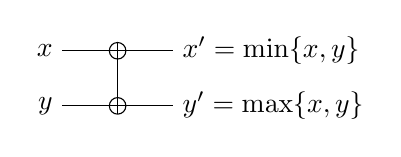
\begin{tikzpicture}[scale=0.7]
    % Draw horizontal lines for x and y
    \draw (-1,1) -- (1,1); % Line for x
    \draw (-1,0) -- (1,0); % Line for y
    
    % Draw vertical line connecting the comparator
    \draw (0,1.15) -- (0,-0.15);
    
    % Draw circles
    \draw (0,1) circle (0.15);
    \draw (0,0) circle (0.15);
    
    % Labels
    \node[left] at (-1,1) {$x$};
    \node[left] at (-1,0) {$y$};
    \node[right] at (1,1) {$x' = \min\{x, y\}$};
    \node[right] at (1,0) {$y' = \max\{x, y\}$};
\end{tikzpicture}
\end{center}

\begin{center}
    \begin{tikzpicture}[scale=0.7]
    % block
    \node[draw, rectangle, minimum width=1.6cm, minimum height=1.2cm] (blk) 
    {\color{red}$\ominus BM[2]$};
    
    % inputs
    \draw
    ($(blk.west)+(-1,0.4)$) node[left] {$x$}
    -- ($(blk.west)+(0,0.4)$);
    \draw
    ($(blk.west)+(-1,-0.4)$) node[left] {$y$}
    -- ($(blk.west)+(0,-0.4)$);
    
    % outputs, shifted up/down by 0.3 units
    \draw
    ($(blk.east)+(0,0.4)$) -- ($(blk.east)+(1,0.4)$)
    node[right] {$x'=\max\{x,y\}$};
    \draw
    ($(blk.east)+(0,-0.4)$) -- ($(blk.east)+(1,-0.4)$)
    node[right] {$y'=\min\{x,y\}$};
\end{tikzpicture}
    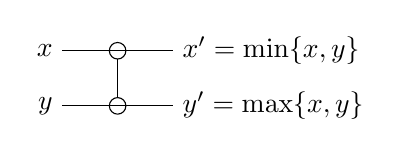
\begin{tikzpicture}[scale=0.7]
    % Draw horizontal lines for x and y
    \draw (-1,1) -- (1,1); % Line for x
    \draw (-1,0) -- (1,0); % Line for y
    
    % Draw vertical line connecting the comparator
    \draw (0,0.85) -- (0,0.15);
    
    % Draw circles
    \draw (0,1) circle (0.15);
    \draw (0,0) circle (0.15);
    
    % Labels
    \node[left] at (-1,1) {$x$};
    \node[left] at (-1,0) {$y$};
    \node[right] at (1,1) {$x' = \min\{x, y\}$};
    \node[right] at (1,0) {$y' = \max\{x, y\}$};
\end{tikzpicture}
\end{center}

Sulla destra una semplificazione in quanto reti con $n = 2$ sono dei comparatori.

Per una rete con $n$ fili, $\oplus BM [n]$, (quindi sequenza bitonica lunga $n$ in ingresso e ordinata in uscita), servono: 
\begin{itemize}
    \item $\log_2 n$ colonne
    
    \item $n/2$ comparatori per colonna
\end{itemize}

Ogni colonna ha comparatori a distanza pari a metà della colonna precedente, a partire da $n/2$ (per $n=16$, prima colonna a distanza $8$, seconda a distanza $4$, \dots, fino a distanza 1 in $\log_2 n$ passi). 

Esempio per rete con $n = 16$:
\begin{center}
    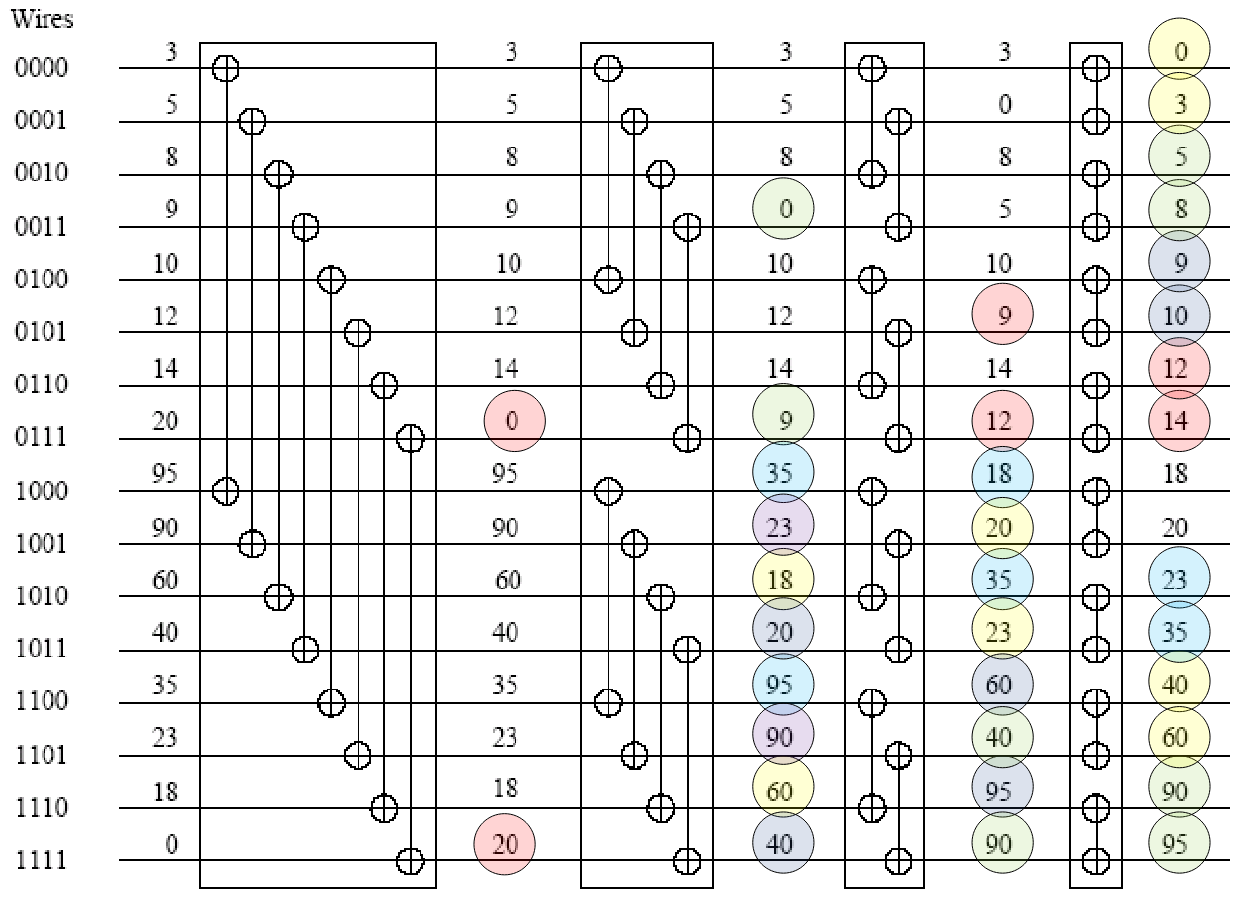
\includegraphics[width=0.79\columnwidth]{img/pattern/n16}
\end{center}

\paragraph{Costruzione di sequenza bitonica:} Con input una sequenza arbitraria, vogliamo ottenere una sequenza bitonica in output. Si può fare alternando i segni dei $BM$.

L'idea è quella di usare una rete con $(\log_2 n) - 1$ colonne: ogni $i$-esima colonna:
\begin{itemize}
    \item prende in input una sequenza bitonica di lunghezza $2^i$, a partire da $i=1$, una sequenza lunga 2 è banalmente bitonica
    
    \item si costruisce una sequenza bitonica lunga $2^{i+1}$ alternando $\oplus BM[2^i]$ con $\ominus BM[2^i]$, da fornire in input alla colonna successiva
\end{itemize}

L'ultima colonna avrà una $\oplus BM [n/2]$ e una $\ominus BM [n/2]$, per creare una sequenza bitonica lunga $n$.

\subsubsection{Ordinamento bitonico}

Si può ordinare una sequenza qualsiasi avendo: 
\begin{itemize}
    \item $(\log n) - 1$ step per costruire una sequenza bitonica a partire dall'input (come visto prima)
    
    \item aggiungere un comparatore $\oplus BM [n]$ alla fine per ordinare la sequenza
\end{itemize}

\paragraph{Complessità:} Per una sequenza lunga $n$, tutte le $\log n$ colonne richiedono: 
\begin{align*}
    T(n) & = T(n/2) + \log (n) \\
    & = \log (n) + \log (n/2) + \dots + 1 \\
    & = \sum_{i=0}^{\log n} i \\
    & = \frac{\log n \left((\log n) + 1\right)}{2} \\
    & = \Theta (\log^2 n) 
\end{align*}

%End L10